\documentclass[a4paper,12pt]{extarticle}
\usepackage[utf8x]{inputenc}
\usepackage[T1,T2A]{fontenc}
\usepackage[russian]{babel}
\usepackage{hyperref}
\usepackage{indentfirst}
\usepackage{listings}
\usepackage{color}
\usepackage{xcolor}
\usepackage{here}
\usepackage{array}
\usepackage{multirow}
\usepackage{graphicx}
\usepackage{amsmath}

\hypersetup{
    colorlinks = false,
    linkbordercolor = {white}
}

\definecolor{string}{HTML}{B40000} % цвет строк в коде
\definecolor{comment}{HTML}{008000} % цвет комментариев в коде
\definecolor{keyword}{HTML}{1A00FF} % цвет ключевых слов в коде
\definecolor{morecomment}{HTML}{8000FF} % цвет include и других элементов в коде
\definecolor{сaptiontext}{HTML}{FFFFFF} % цвет текста заголовка в коде
\definecolor{сaptionbk}{HTML}{999999} % цвет фона заголовка в коде
\definecolor{bk}{HTML}{FFFFFF} % цвет фона в коде
\definecolor{frame}{HTML}{999999} % цвет рамки в коде
\definecolor{brackets}{HTML}{B40000} % цвет скобок в коде

\usepackage{caption}
\renewcommand{\lstlistingname}{Программа} % заголовок листингов кода

\bibliographystyle{ugost2008ls}

\usepackage{listings}
\lstset{ %
	extendedchars=\true,
	keepspaces=true,
	language=Python,						% choose the language of the code
	% Цвета
	keywordstyle=\color{keyword}\ttfamily\bfseries,
	%stringstyle=\color{string}\ttfamily,
	stringstyle=\ttfamily\color{red!50!brown},
	commentstyle=\color{comment}\ttfamily\itshape,
	morecomment=[l][\color{morecomment}]{\#},
	basicstyle=\footnotesize,		% the size of the fonts that are used for the code
	numbers=left,					% where to put the line-numbers
	numberstyle=\footnotesize,		% the size of the fonts that are used for the line-numbers
	stepnumber=1,					% the step between two line-numbers. If it is 1 each line will be numbered
	numbersep=5pt,					% how far the line-numbers are from the code
	backgroundcolor=\color{white},	% choose the background color. You must add \usepackage{color}
	showspaces=false				% show spaces adding particular underscores
	keywordstyle=color{blue}\bfseries, 
	showstringspaces=false,			% underline spaces within strings
	showtabs=false,					% show tabs within strings adding particular underscores
	frame=single,          		% adds a frame around the code
	tabsize=2,						% sets default tabsize to 2 spaces
	captionpos=t,					% sets the caption-position to top
	breaklines=true,				% sets automatic line breaking
	breakatwhitespace=false,		% sets if automatic breaks should only happen at whitespace
	escapeinside={\%*}{*)},			% if you want to add a comment within your code
	postbreak=\raisebox{0ex}[0ex][0ex]{\ensuremath{\color{red}\hookrightarrow\space}},
	texcl=true,
	inputpath=listings,                     % директория с листингами
}

\usepackage[left=2cm,right=2cm,
top=2cm,bottom=2cm,bindingoffset=0cm]{geometry}

%% Нумерация картинок по секциям
\usepackage{chngcntr}
\counterwithin{figure}{section}
\counterwithin{table}{section}

%%Точки нумерации заголовков
\usepackage{titlesec}
\titlelabel{\thetitle.\quad}
\usepackage[dotinlabels]{titletoc}

%% Оформления подписи рисунка
\addto\captionsrussian{\renewcommand{\figurename}{Рисунок}}
\captionsetup[figure]{labelsep = period}

%% Подпись таблицы
\DeclareCaptionFormat{hfillstart}{\hfill#1#2#3\par}
\captionsetup[table]{format=hfillstart,labelsep=newline,justification=centering,skip=-10pt,textfont=bf}

%% Путь к каталогу с рисунками
\graphicspath{{fig/}}

\begin{document}	% начало документа

% Титульная страница
%\begin{titlepage}	% начало титульной страницы

	\begin{center}		% выравнивание по центру

		Санкт-Петербургский Национально Исследовательский Университет\\
		информационных технологий, механики и оптики \\
		Кафедра систем управления и информатики\\[3cm]
		% название института, затем отступ 6см
		
		\huge \textbf{РЕФЕРАТ}\\[0.5cm]
		\large Электромеханические системы\\[0.1cm]
		\large Система автоматического управления квадракоптера Parrot ARDrone 2.0\\[2cm]

	\end{center}


	\begin{flushright} % выравнивание по правому краю
%		\begin{minipage}{0.5\textwidth} % врезка в половину ширины текста
%			\begin{flushleft} % выровнять её содержимое по левому краю

				\large Выполнили студенты группы P3335\\
				\large А.М. Зенкин\\[0.5cm]
				\large К.В. Карпов\\[0.5cm]
				
				\large Принял  к.т.н., доцент кафедры СУиР\\
				\sign[4cm]\large  М.С. Чежин\\
				\large Оценка: \sign\\
				«\underline{\hspace{0.7cm}}» \underline{\hspace{2cm}} \the\year г.

%			\end{flushleft}
%		\end{minipage}
	\end{flushright}
	
	\vfill % заполнить всё доступное ниже пространство

	\begin{center}
	\large Санкт-Петербург\\
	\large \the\year % вывести дату
	\end{center} % закончить выравнивание по центру

\thispagestyle{empty} % не нумеровать страницу
%\end{titlepage} % конец титульной страницы
\newpage


% Содержание
% Содержание
\renewcommand\contentsname{\centerline{Содержание}}
\tableofcontents
\thispagestyle{fancy}
\newpage




\section{Типы заземляющих устройств}
Для заземления электроустановок используется заземляющее устройство (рис. 3.8), состоящее из заземлителя – одиночного или группы заземлителей 1, конструктивно объединенных соединительной полосой 2, размещаемых в земле, и заземляющего проводника 3, соединяющего заземляемую установку 4 через проложенную по стенам помещения магистраль заземления 5 с заземлителем.

Для присоединения заземляющего проводника на корпусе установки должен быть предусмотрен элемент для заземления – болт 6 (винт, шпилька), выполненный из металла, стойкого к коррозии. Возле болта должен быть нанесен нестираемый при эксплуатации знак заземления 7.


\begin{figure}[H]
	\begin{center}
		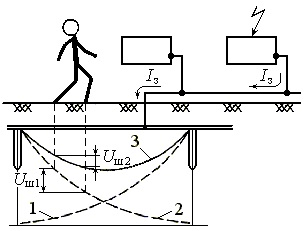
\includegraphics[scale=1.4]{pic_1.jpg}
		\caption{ - напряжение шага при одиночном и групповом заземлителе} 
		\label{pic:pic_1} % название для ссылок внутри кода
	\end{center}
\end{figure}

В качестве искусственных заземлителей, располагаемых в земле чаще всего вертикально, используются стальные трубы диаметром 5 – 6 см с толщиной стенки не менее 3,5 мм или уголки с толщиной полок не менее 4 мм и размерами от 40x40 мм до 60x60 мм длиной 2,5 – 3 м.

Различают два типа заземляющих устройств: выносное и контурное.

В выносном заземляющем устройстве заземлитель вынесен за пределы площадки, на которой размещено заземляемое электрооборудование. Такой тип заземляющего устройства применяют только при малых значениях тока замыкания на землю.

В контурном заземляющем устройстве одиночные вертикальные зазем-лители располагают по контуру (периметру) площадки, на которой нахо-дится заземляемое оборудование (см. рис. 3.9), или заземлители распреде-ляют по всей площадке по возможности равномерно.

\begin{figure}[H]
	\begin{center}
		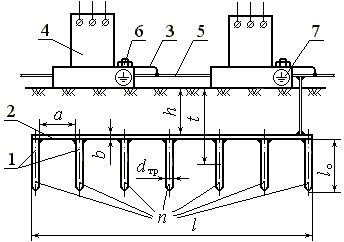
\includegraphics[scale=1.4]{pic_2.jpg}
		\caption{ - устройство защитного заземления} 
		\label{pic:pic_1} % название для ссылок внутри кода
	\end{center}
\end{figure}

1 – электроустановка; 2 – заземляющий проводник; 3 – магистраль заземления; 4 – перемычка; 5 –заземлитель; 6 – соединительная полоса
\\

Безопасность при использовании контурного заземляющего устройства обеспечивается не только уменьшением потенциала заземленного оборудо-вания, но и выравниванием и повышением потенциала на поверхности за-щищаемой территории путем размещения одиночных заземлителей на определенном расстоянии друг от друга (менее 40 м).

Расчёт контурного заземляющего устройства сводится к определению количества заземлителей, длины соединительной полосы и схемы размещения заземлителей в земле на защищаемой территории, при которых сопротивление заземляющего устройства и напряжение прикосновения не превысят допустимых значений.

\section{Входные данные}

№ варианта: 3\\
Вид заземлителя: Труба; Вид соедин.полосы: Полоса;\\
h = 0, м; $l_0$ = 2.9, м; $d_\text{тр}$ = 40, мм; b = 40, мм; a = 4.5, м;\\
$k_\text{сез}$ = 1.3; $\eta_\text{з}$ = 0.65; $\eta_\text{п}$ = 0.3; $\rho$ = 70, Ом*м \\ 

\section{Расчёт защитного заземления}

Произвести расчёт параметров контурного
заземляющего устройства для защитного заземления электроустановок по
следующим исходным данным: заземлители – стальные трубы диаметром
50 мм, длиной 3 м забиваются в землю на глубину 0,6 м от ее поверхности;
соединительная полоса – стальная полоса шириной 40 мм; грунт – глина,
удельное сопротивление которой ρ = 60 Ом·м. Расстояние между двумя
соседними заземлителями 4 м; значения коэффициентов: к сез = 1,4; η з = 0,7;
η п = 0,4.

\subsection{Определяем сопротивление одного вертикального заземлителя растеканию тока в земле:}

\begin{equation}
    \begin{split}	
        &R_\text{pipe}=\frac{\rho_p}{2\pi \cdot l_0}\cdot ln \frac{4 l_0}{d_{pipe}} = \frac{1.3 \cdot 70}{2\pi \cdot 2.9}\cdot ln \frac{4 \cdot 2.9}{40} = 28.331\; Om;\\
    \end{split}
\end{equation}

\subsection{Определяем необходимое число вертикальных заземлителей n:}

\begin{equation}
    \begin{split}	
        &n=\frac{R_0}{R_{z} \cdot \eta_{z}} = \frac{28.331}{4 \cdot 0.65} = 10.896\; pcs;\\
    \end{split}
\end{equation}

Полученное значение следует округлять в меньшую сторону до целого числа. Принимаем число заземлителей n = 10 шт.;

\subsection{Рассчитываем длину соединительной полосы l:}

\begin{equation}
    \begin{split}	
        &l = 1.05\cdot an = 1.05\cdot 4.5\cdot 10 = 47.25\; м;\\
    \end{split}
\end{equation}

\subsection{Определяем сопротивление соединительной полосы растеканию тока:}

\begin{equation}
    \begin{split}	
        &R_{p} = \frac{\rho_p}{2 \pi \cdot l} ln \frac{2 l }{0.5 \cdot b} =\frac{1.3 \cdot 70}{2 \pi \cdot 47.25} ln \frac{2\cdot 47.25 }{0.5 \cdot 40} = 0,476\; Om;\\
    \end{split}
\end{equation}

\subsection{Рассчитываем полное сопротивление заземляющего устройства:}

\begin{equation}
    \begin{split}	
        &R_{zy} = \frac{R_{pipe}\cdot R_p}{R_z \eta_{p} + nR_p\cdot \eta_{z}} = \frac{28.331\cdot 0.476}{4\cdot 0.3 + 10\cdot 0.476p\cdot 0.65} = 1.164\; Om;\\
    \end{split}
\end{equation}

Расчёт считаем законченным, так как сопротивление проектируемого заземляющего устройства менее 4 Ом, что соответствует требованиям ПУЭ.



\end{document}
